
%% bare_conf.tex
%% V1.3
%% 2007/01/11
%% by Michael Shell
%% See:
%% http://www.michaelshell.org/
%% for current contact information.
%%
%% This is a skeleton file demonstrating the use of IEEEtran.cls
%% (requires IEEEtran.cls version 1.7 or later) with an IEEE conference paper.
%%
%% Support sites:
%% http://www.michaelshell.org/tex/ieeetran/
%% http://www.ctan.org/tex-archive/macros/latex/contrib/IEEEtran/
%% and
%% http://www.ieee.org/

\documentclass[10pt, conference]{IEEEtran}

\usepackage{booktabs}
\usepackage{cite}
\usepackage{color}
\usepackage{enumerate}
\usepackage[utf8]{inputenc}
\usepackage{tikz}
\usepackage{multicol}
\usepackage{multirow}

%\usepackage[brazil]{babel}
%\usepackage[cmex10]{amsmath}
%\usepackage{algorithmic}
%\usepackage{array}
%\usepackage{mdwmath}
%\usepackage{mdwtab}
%\usepackage{eqparbox}
%\usepackage[tight,footnotesize]{subfigure}
%\usepackage[caption=false]{caption}
%\usepackage[font=footnotesize]{subfig}
%\usepackage[caption=false,font=footnotesize]{subfig}
%\usepackage{fixltx2e}
%\usepackage{stfloats}
\usepackage{url}



\newif\ifComments

% To turn comments OFF simply comment out the \Commentstrue line
\Commentstrue

\ifComments
\newcommand{\luiz}[1]{\noindent\textcolor{cyan}{LUIZ: {#1}}}
\newcommand{\mario}[1]{\noindent\textcolor{cyan}{MARIO: {#1}}}
\newcommand{\rem}[1]{\noindent\textcolor{magenta}{REMOVED: {#1}}}
\newcommand{\new}[1]{\noindent\textcolor{blue}{NEW: {#1}}}
\newcommand{\rev}[1]{\noindent\textcolor{red}{REVISE: {#1}}}
\else
\newcommand{\luiz}[1]{}
\newcommand{\mario}[1]{}
\newcommand{\rem}[1]{}
\newcommand{\new}[1]{#1}
\newcommand{\rev}[1]{#1}
\fi

% correct bad hyphenation here
\hyphenation{}
\usetikzlibrary{shapes.geometric, arrows}

\tikzstyle{activity} = [rectangle, rounded corners, minimum width=5cm, minimum 
height=1cm,text centered, draw=black, fill=white]
\tikzstyle{io} = [trapezium, trapezium left angle=70, trapezium right angle=110, minimum width=3cm, minimum height=1cm, text centered, draw=black, fill=blue!30]
\tikzstyle{process} = [rectangle, minimum width=3cm, minimum height=1cm, text centered, text width=3cm, draw=black, fill=orange!30]
\tikzstyle{decision} = [diamond, minimum width=3cm, minimum height=1cm, text centered, draw=black, fill=green!30]
\tikzstyle{arrow} = [thick,->,>=stealth]
\tikzstyle{line} = [draw, -latex']


\begin{document}

\title{Machine Learning Based Prediction of Change Request Severity Level: Experimental Results}

\author{\IEEEauthorblockN{Author1}
\IEEEauthorblockA{Affiliation1}
\and
\IEEEauthorblockN{Author2}
\IEEEauthorblockA{Affiliation2}
}

\maketitle

\begin{abstract}
In the context of Change Request (CR) systems, the severity level of a change request is considered a critical variable when planning software maintenance activities, indicating how soon a CR needs to be addressed. However, the severity level assignment remains primarily a manual process, mostly depending on the experience and expertise of the person who has reported the CR. In this paper, we present preliminary findings of ongoing research aimed to predict the severity level of a CR by analyzing its long description, using text mining techniques and Machine Learning (ML) algorithms. Best results were obtained with a classifier based on the Random Forest ML algorithm. This classifier can predict whether the severity level will change (accuracy of 93.681\%) and if it will increase or decrease (accuracy of 93.440\%). However, preliminary results were not as good when predicting the final severity level in an imbalanced data scenario. 

\end{abstract}

\begin{IEEEkeywords}
software maintenance; change request systems; machine learning; random forest.
\end{IEEEkeywords}


% For peer review papers, you can put extra information on the cover
% page as needed:
% \ifCLASSOPTIONpeerreview
% \begin{center} \bfseries EDICS Category: 3-BBND \end{center}
% \fi
%
% For peerreview papers, this IEEEtran command inserts a page break and
% creates the second title. It will be ignored for other modes.
\IEEEpeerreviewmaketitle

\mario{GERAL: passar a usar acronimo CR no restante do artigo. Faltam comparacoes dos nossos resultados com a literatura. Figuras e tabelas incluidas e citadas devem ser explicadas, pelo menos um pouco, caso contrario o revisor pode acha-la desnecessaria. Nao usar expressoes absolutas: the best, the worst, the fastest, etc. Evitar primeira pessoa. Voz passiva ok, mas ordem direta eh melhor.  Nunca dizer: in section xx we present.... Diga: section xx presents. A conversar com MC: comentar sobre a estrutura hierarquica do texto, com intro-desenv-concl, em cada nivel. Indicar significado das siglas na primeira ocorrencia. Indicar referencia a tecnicas, metodos, artigos, quando citados. Ao citar texto ipsis literis, se for longo, colocar entre aspas e dar o devido crédito. Se preferir usar de passagem, reescreva para nao haver acusacao de plagio. Deve haver um espaco antes de abrir parenteses; ha varios casos sem espaco.  Nao usar giria nem apostrofe em verbo isn't e sim is not, etc.}


\section{Introduction}
Change Request (CR) systems \rem{has been performed a critical} \new{have played a major} role in maintenance process in many software development settings, both in Close Source Software (CSS) and in Open Source Software (OSS) scenarios. \rem{Mainly in the latter}\new{This is specially true in OSS}, which is characterized by the existence of many of users and developers with \rem{distinct expertise levels} \new{different levels of expertise} spread out around the world, who might \rem{register or deal with any amount of} \new{create or be responsible for dealing with several} change requests\cite{Cavalcanti2014}. 

A user interacts with a CR system often through a simple mechanism called CR form. This form enables him to request changes, to report bugs or to ask for support in a software product\cite{Sommerville2010}. Initially, he or she should inform a short description, a long description, a type (e.g. bug, new feature, improvement, and task) and an associated severity level (e.g. blocker, critical, major, minor and trivial)\rem{ for his or her solicitation} \mario{evite a palavra solicitation}. Subsequently, a development team member will review this request and, case it is not refused for some reason (e.g. request duplication), he or she will complete the information in CR form, indicating, for example, its priority and the person responsible for accomplishing it. \mario{importante usar terminologia e jargao do ramo: acho que aqui nao eh accomplish e sim assigned for the CR; verificar em outros artigos}

The severity level information is recognized as a critical variable in the equation to estimate a prioritization of change request \rem{prioritization}\cite{Tian2012} \mario{repetido}. \rem{Consequently, it can be a decisive factor how soon it needs to be fixed\cite{Lamkanfi2010}}\new{It defines how soon the CR needs to be addressed\cite{Lamkanfi2010}}. However, the severity level assignment remains mostly a manual process which relies only on the experience and expertise of the person who has opened the CR \cite{Cavalcanti2014, Tian2012, Lamkanfi2010}. \rem{So, it may allow a high degree of subjectivity and, consequently,}\new{As a consequence, it is a process with high degree of subjectivity, and} it may be quite error-prone. 

The number of CRs in large and medium software OSS projects\cite{Lamkanfi2011} is frequently very large. Severity level shifts throughout CR lifecycle (Figure \ref{fig:cr-life-cycle}) \rem{could cause relevant impact on}\new{may adversely affect} planning of maintenance activities. For example, the maintenance team could be assigned to address less significant CRs before the most important ones. \mario{voce cita a figura mas nao fala nada dela --------- REMOVER}

\mario{Aqui ha um salto de raciocinio. Imagine como voce faria esta transicao oralment}

Machine Learning (ML) techniques have been successfully applied in solving real problems in many areas of knowledge, including those related to CR systems, such as duplication and assignment of CR\cite{Cavalcanti2014}. However, the accuracy of ML algorithms may be affected by imbalanced datasets \cite{Chawla2009} \textemdash  a recurring critical problem in CR repositories\cite{Tian2015}. For example, more than 60\% of CRs may have a ``major" severity level.\mario{veja a sintaxe para matching double quotes} 


\begin{figure}[hbt!]  
  \centering
  \begin{tikzpicture}[node distance=1.5cm]
    \node (a1) [activity] {Open};
    \node (a2) [activity, below of=a1] {In Progress};
    \node (a3) [activity, below of=a2] {Resolved};
    \node (a4) [activity, below of=a3] {Closed};
    \node (a5) [activity, below of=a4] {Reopened};
    
    \draw [arrow] (a1) -- (a2);
    \draw [arrow] (a2) -- (a3);
    \draw [arrow] (a3) -- (a4);
    \draw [arrow] (a4) -- (a5);
    \draw [arrow] (a5.east)  -- ++(1.5,0) |- (a1.east);
    \draw [arrow] (a3.west)  -- ++(-1.5,0) |- (a5.west);
  \end{tikzpicture}
  \caption{CR life cycle\cite{Sommerville2010}.}
  \label{fig:cr-life-cycle}
\end{figure}

\mario{aqui deveria entrar a motivacao. Motivacao sempre e: melhorar o desempenho de algo; ou suprir um falha de algo. Vc poderia por ex dizer: muitos estudam CR com ML mas nao ha um comparativo entre algoritmos; ou o desempenho esta muito baixo; ou a melhoria com relacao a predicao manual nao eh medida. E preciso justificar porque vc fez o trabalho. Sugestao durante a reuniao: ha muitos trabalhos mas ainda nao satisfatorios. Ha espaco para melhoria e criacao de ferramenta.}

In this context, our goal is to indicate the best ML classifier to predict the severity level of a CR in an imbalanced data scenario, based on the assessment the accuracy of three traditional ML algorithms: Neural Networks (NN), Random Forest (RF) and Support Vector Machine(SVM). \mario{discutir em reuniao: eh isso mesmo? Se sao so 3, entao nao eh the best. OUTRA COISA: eu daria destaque para o goal. Eh comum numerar G1, G2, e depois abaixo RQ1, RQ2, etc, inclusive relacionando-as entre si.}

\rem{To systematize our evaluation, our experiments should answer the following research questions}\new{The research questions of this study are:}

\begin{enumerate}[RQ 1:]
  \item \textit{Will CR severity level change during its lifecycle?} we have investigated the accuracy of the classifiers to answering a binary response question: if CR will remain its severity level or it will change.
  \item \textit{Will the change request severity level increase, decrease or remain the same during its lifecycle}? we have investigated the accuracy of the classifiers to answering a ternary response question: if CR will remain, increase or decrease its severity level.
  \item \textit{What will the change request severity level at the end of its lifecycle?} Finally, we have investigated the accuracy of the classifiers to answering a question with more than three responses.
\end{enumerate}

\mario{\\ A lista de RQ nao deve misturar as perguntas com a estrategia para seu encaminhamento. Uma possibilidade seria (depois da lista) justificar a escolha delas.}

This paper aims to deliver the following contributions\mario{Vamos conversar sobre isto na reuniao. Ver artigos semelhantes da MSR}: 

\begin{enumerate}
  \item Indicate the performance of three ML algorithms to answering questions with two, three or more responses in an imbalanced scenario.  
  \item Suggest another way to measure the performance of ML algorithms in imbalanced data scenario besides the traditional forms used for this purpose.
  \item Advance the researches on the topics discussed in this article.
\end{enumerate}

The structure of this paper is as follows. Section \ref{sec:relatedwork} presents related work that are relevant to our research. Section \ref{sec:background} provides the information background about CR systems, text mining and machine learning techniques necessary to understand our approach. Section \ref{sec:experiment} describes our work. Section \ref{sec:discussion} presents final findings and discussion. \rem{Finally, we conclude and discuss future work in Section 6}\new{Finally, Sections \ref{threats} and \ref{sec:conclusion} present the threats to validity of this research, and conclusions and  future work, respectively}\mario{deixei aqui p vc ver um exemplo de trocar voz passiva pela ordem direta, e tbem remover a primeira pessoa. Ja mudei no resto deste paragrafo}.


\section{Related Work}\label{sec:relatedwork} \mario{usar label e ref para ref cruzada}

\mario{aqui vc entrou de chofre. Precisaria fazer uma introducao}

Menzies\cite{Menzies2008} have developed a method, named SEVERIS (SEVERity ISsue assessment), for evaluating the severity of changes requests. SEVERIS is based on common text mining techniques (e.g. tokenization, stop word removal, stemming, Tf*Idf and InfoGain) and on the data mining techniques (e.g. RIPPER). The method was applied to five projects managed by the Project and Issue Tracking System (PITS). - an issue tracker system used by NASA. \mario{Quais foram os resultados ou conclusoes? Em que medida isso eh util p nosso trabalho ou diferente dele?} \mario{Em toda a secao vc cita varias tecnicas e metodos. Discutir necessidade de referencia}

Lamkanfi et al.\cite{Lamkanfi2010} have developed an approach to predict severity level of a CR based on text mining algorithms (tokenization, stop word removal, stemming) and on the Naïve Bayes machine learning algorithm. They have been validated their approach over from three open source project Mozilla, Eclipse, and GNOME and they accomplished that a training set with approximately 500 change requests per severity degree are enough to predict it with a reasonable accuracy. In another following work, Lamkanfi et al.\cite{Lamkanfi2011}, these authors compared the accrual of four machine-learning algorithms (Naïve Bayes Multinomial, K-Nearest Neighbor, and Support Vector Machine). They have been concluded that Naïve Bayes Multinomial gave superior performance compared to the others proposed algorithms.

Valdivia et al.\cite{ValdiviaGarcia2014} have characterized blocking bugs in six open source projects and proposed a model to predict them. Their model was composed of 14 distinct factors or features (e.g. the textual description, location the bug is found in and the people involved with the bug). Based on these factors they build decision trees for each project to predict whether a bug will be a blocking bug or not. Then, they analyze these decision trees to determine which factors best indicate these blocking bugs. 

\section{BACKGROUND} \label{sec:background} 
\rem{In this section, we describe de change request process. Next we explain the common approach to pre-processing textual documents, and lastly, we highlight the three ML algorithms: Neural Networks, Random Forest and SVM.}\new{This section presents basic background material: change request process and Change Request Systems (Section \ref{subsec:crs}; usual approaches to pre-processing textual documents and text mining (Section \ref{subsec:texmining}); and a brief description of three Machine Learning algorithms used in this research, Neural Networks, Random Forest and SVM (Section \ref{subsec:ml}). Finally, typical Evaluation Metrics are presented (Section \ref{subsec:metrics}). }

\subsection{Change Request Systems}		\label{subsec:crs}
Change Request systems\cite{Pressman2009} are software employed to keep the recording and tracking information of requests for modifications, bug fixes, and support that could occur during the software life cycle. 

Although there is no \rem{a common sense} \new{consensus} regarding terminology or the amount of information that users must fill in to complete his requisition among popular CR systems (e.g. Bugzilla, Jira, and Redmine)\cite{Tian2012}, typically, \rem{they shall fill in a form containing at least the} \new{a CR form contains the} following attributes shown in Table \ref{tab:commom_attributes_cr_form}. 

\begin{table}[!ht]
	% increase table row spacing, adjust to taste
	\renewcommand{\arraystretch}{1.3}
	\caption{Commom attributes in the CR forms.}
	\label{tab:commom_attributes_cr_form}
	\centering
	\begin{tabular}{|l|p{6cm}|}
		\hline
		Type & Type of request (e.g. bug, new feature, improvement, and new feature)\\
		\hline
		Title & Short description of request in one line.\\
		\hline
		Description & Long and detailed description of request in many lines. It could include source code snippets and stack tracing reports.\\
		\hline
		Severity & Level of severity of request (e.g. blocker, critical, major, minor and trivial).\\
		\hline 
	\end{tabular}
\end{table}

Once the request has been registered by the user, the development team will assess it and, if it not canceled for some reason (e.g. duplication), \rem{they will complement the information with, for example, } \new{will assign the CR to the person responsible for handling it. The development team may include additional information at any time.} All these data are stored in a repository, keeping relevant historical data about the system under development. \mario{este material eh muito basico. Talvez seja desnecessario. Colocar so o que nao eh obvio e eh necessario para o entendimento. Por ex: atributos, problemas de terminologia, historico de alteracao.}

\subsection{Text Mining}   \label{subsec:texmining}
Text mining is the process to convert unstructured text into a structure suited to analysis\cite{Feldman2007}. It is composed of three basic activities\cite{Williams2011}: tokenization, stop word removal and stemming.

Tokenization is the action to parsing a character stream into a sequence of tokens by splitting the stream at delimiters. In this context, a token is defined as a block of text or a string of characters (without delimiters such as spaces and punctuation) that is recognized as a useful portion of the unstructured data.

Stop words eliminates commonly used words that do not provide relevant information to a particular context, including prepositions, conjunctions, articles, common verbs, nouns, pronouns, adverbs, and adjectives.

Stemming is the process stemming is the process of reducing or normalizing inflected (or sometimes derived) words to their word stem, base form—generally a written word form (e.g. “working” and worked into work). \mario{Vc copiou algum texto ipsis literis? Caso afirmativo reescreva. Isso vale para toda esta secao.}

\subsection{Machine Learning}   \label{subsec:ml}
\rem{The machine learning}\new{Machine Learning} \mario{So use o the se estiver falando daquele especifico ML.} is considered a part of artificial intelligence area whose the primary purpose is to resolve a given problem using experience or example data\cite{Surya2016}. It can be seen as an improvement over a set of techniques or methodologies which can make a computer to learn by the study of data sets.

\mario{Fazer introducao aqui. Enumerar algumas tecnicas e citar que ira descrever x, y, z (ref subsec) por serem mais relevantes nesta area}

% TODO: colocar referências.
\subsubsection{Neural Networks}   \label{subsubsec:nn}
Neural Network is a learning algorithm that is inspired by the structure and functional aspects of biological neural networks\cite{Russell2010}. Computations are structured regarding an interconnected group of artificial neurons, processing information using a connectionist approach to computation. 

Modern neural networks are non-linear statistical data modeling tools. They are usually used to model complex relationships between inputs and outputs, to find patterns in data, or to capture the statistical structure in an unknown joint probability distribution between observed variables.

\subsubsection{Random Forest}     \label{subsubsec:rf}
The Random Forest algorithm\cite{Breiman2001} relies on two core principles: (i) in the creation of hundreds of decision trees and the joining them into a single model; and (ii) in the closing decision based on the ruling of the majority of the forming trees which are treated as equals.

A random forest model is considered a suited alternative for model construction for a many of reasons\cite{Williams2011} 

\begin{itemize}
  \item Requires little or no data preprocessing, no data normalization and it is resilient to outliers.
  \item Requires no variable selections because the algorithm does its own.
  \item Models resultants from each tree in the forest tend not to overfit to the training dataset because they are built using two levels of randomness (observations and variables).
\end{itemize}

\subsubsection{Support Vector Machine}		\label{subsubsec:svm}
Support Vector Machine is considered the most popular algorithm for supervised learning and an excellent first method to testing\cite{Russell2010}. It is a set of related supervised learning methods used for classification and regression. Each example in a set of training data is marked as belonging to one of two categories an the SVM algorithm builds a model that predicts whether a new example falls into one category or the other. 

\subsection{Evaluation Metrics}	\label{subsec:metrics}
From Information Retrieve (IR) discipline, \mario{referencia?} the three most common performance measures for evaluating the accuracy of classification algorithms are precision, recall, and F-measure\cite{Feldman2007}. 

\textbf{Recall}. The recall for a class can be defined as the percentage of correctly classified observations among all observations belonging to that class. It can be thought of as a measure of a classifiers completeness. More formally\cite{Facelli2015}: the recall is the number of True Positives (TP) divided by the number of True Positives (TP) and the number of False Negatives (FN), where the TP and FN values are derived from the confusion matrix. A low recall indicates many False Negatives\cite{Zhao2013}. \mario{Talvez valha a pena mostrar a matriz de confusao.}

\textbf{Precision}. The precision is the percentage of correctly classified observations among all observations that were assigned to the class by the classifier. It can be thought of as a measure of classifier exactness. More formally\cite{Facelli2015}: the precision is the number of True Positives (TP) divided by the number of True Positives and False Positives (FP), as well as TP and FN, FP also comes from the confusion matrix. A low precision can also indicate a large number of False Positives\cite{Zhao2013}.

\textbf{F-measure}. F-measure conveys the balance between the precision and the recall and combines the two measures in an ad hoc way\cite{Feldman2007, Zhao2013}.F-measure can be calculated using the formula $2*((precision*recall))/(precision+recall)$. 

\mario{\\Nao revisei ML e Evaluation}

\section{Experiment} \label{sec:experiment}
\rem{In this section, we describe our approach which was conducted following the steps in Figure \ref{fig:methodology} } \new{This section presents the design and execution of the experimental work, according to the steps depicted in Figure \ref{fig:methodology}, reflecting the typical methodology used in ML studies. } \mario{Nesta secao, ficou faltando abordar claramente o planejamento da execucao. Dizer, por exemplo quais escolhas e dimensionamentos foram tomados e por que. Por exemplo, a figura (talvez desnecessaria) poderia ter sido mencionado que eh a sequencia tipica de passos em tarefas de ML, conforme referencia. Lembre-se: em trab academico, toda afirmacao ou decisao deve estar fundamentada na literatura ou deve ser provada-explicada. Sugestao apos reuniao: remover figura, MC ver se pode melhorar a parte de planejamento em cada passo, explicar escolhas.}

\begin{figure}[!ht]	
	\centering
	\begin{tikzpicture}[node distance=1.5cm]
		\node (a1) [activity] {Data Collection};
		\node (a2) [activity, below of=a1] {Preprocessing};
		\node (a3) [activity, below of=a2] {Training and Testing};
		\node (a4) [activity, below of=a3] {Results Evaluation};
		
		\draw [arrow] (a1) -- (a2);
		\draw [arrow] (a2) -- (a3);
		\draw [arrow] (a3) -- (a4);;
		%%\draw [arrow] (a4.east)  -- ++(2.5,0) |- (a1.east);
	\end{tikzpicture}
	\caption{Methodology used in this study.}
	\label{fig:methodology}
\end{figure}

\subsection{Data Collection}. 
\mario{Dizer porque escolheu o Hadoop. Alias, falta alinhar com a nossa escolha de FLOSS.} We have created our dataset to training and testing the machine learning from the changes requests data collected from Apache HADOOP project. According to [hadoop.apache.org], HADOOP is "framework that allows for the distributed processing of large data sets across clusters of computers using simple programming models. It is considered a specialized and complex OSS project with many users with distinct expertise level. This fact has provided us access to change requests, in XML format, with different levels of information. From CR's long descriptions with few character lines to ones with many lines, including even code snippets and exception stack trace.

The users of HADOOP have registered and stored their CRs via Jira
software[\url{https://www.atlassian.com/software/jira}]. To collect these data, we have organized its extraction into two steps: (i) the copying of CR basic data (e.g. status and resolution) in XML; and (ii) the copying of CR changes histories in HTML, both from HADOOP web site[\url{http://issues.apache.org}]. About 10\% of the CRs collected in this process changed at least once their level of severity.

We collected CR published from February 01, 2006 to January 18, 2017.  We only retrieved requests from the common module which identifier started with HADOOP. The total number of records retrieved after preprocessing was 7129 change requests. Figure \ref{fig:ds_distribution} shows three charts with requests distribution by severity level and severity level changes.

\begin{figure*}[!hbt]
  \label{fig:ds_distribution}
  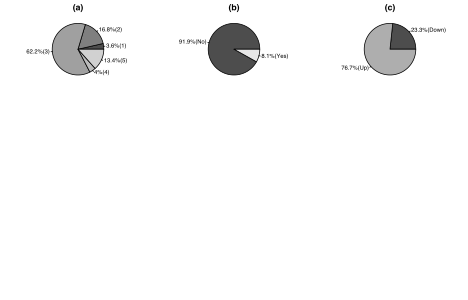
\includegraphics{figures/ds_distribution.pdf}
  \caption{Dataset distribution by severity level.}
\end{figure*}


The graph (a) shows that of 7129 change requests, 3.6\% had severity 1 (trivial); 16.8\% had severity 2 (minor); 62.2\% had severity 3 (major), 4.0\% had severity 4 (critical), And 13.4\% had severity 5 (blocker). The graph (b) shows that 91.9\% of them haven't changed their severities levels and 8.1\% have changed. And the graph (c) reveals that of the 8.1\% which changed their severity, 23.3\% decreased it, and 76.7\% increased it. We can note that dataset is clearly imbalanced.


\subsection{Preprocessing}
The CR data stored in XML and HTML files which we have copied from HADOOP website weren't in tidy data\cite{DeJonge2013}, i.e., it wasn't in appropriated format to train and test the machine learning. To convert it to this suitable format, we have coded and run scripts written in language R. These scripts execute the following tasks:
\begin{itemize}
 \item Extraction from files many features: the key, the type, the status, the resolution and the long description of CR's;
 \item Filtering the only CR's with status equals to Closed and resolution equals to Fixed and Implemented. 
 \item Merging the CR's features with history data to discover what CR's have changed its severity level and if there was increasing or decreasing in this level.
 \item Extraction from the long description initially the one hundred the most frequent words and convert them into features for each CR.
 \item Classifying the CR's in ascending chronological date. 
\end{itemize}


\subsection{Training and testing}. 

To train and test de machine learning, we have partitioned the dataset generated after preprocessing in two distinct pieces: one part for training with 60\% of the dataset and one part for testing with 40\% of the dataset. In the training phase, we have used the 3-fold cross-validation technique to choose the best values for hyperparameters for each classifier algorithm to use them in the test phase. 


\section{Findings and Discussions}  \label{sec:discussion}

\subsection{RQ1: Will the change request severity level change during its lifecycle?}

The RQ1 is a simple binary problem, i.e., a question whose answer is true or false. The Table \ref{tab:metrics_for_rq1} shows the performance (in percentage) of the classifiers to predict the response to this issue.

% 0.9179235
\begin{table}[!ht]
	\renewcommand{\arraystretch}{1.3}
	\caption{Classifiers Performances on RQ1.}
	\label{tab:metrics_for_rq1}
	\centering
	\begin{tabular}{|l|c|c|c|}
		\hline
		Classifier & Precision & Recall & F-Measurement\\
		\hline 
		NN & 93,381 & 98,015 & 95,642\\
		\hline
		RF & 93,801 & 99,923 & 96,765\\
        \hline
		SVM & 93,727 & 99,809 & 96,627 \\
		\hline
		
	\end{tabular}
\end{table}

We tested the classifiers with 2851 (40\% of 7129) change requests: 2620 have changed their severity level, and 231 haven't changed their severity level. We can observe that the three classifiers performed very closely. However, the Random Forest classifier have achieved a F1-Measure somewhat better than the two others.

Regarding the Random Forest classifier we have done one step further, we have investigated its performance relating to the number of hits and errors made in answer to RQ1. The Figure \ref{fig:rf_performance_for_q1} indicates that its accuracy was 93.681\% (2676 divide by 2851). 

\begin{figure}[!hbt]
  \label{fig:rf_performance_for_q1}
  \includegraphics[width=0.5\textwidth, height=0.42\textwidth]{figures/rf_performance_for_q1.pdf}
  \caption{Performance of Random Forest for RQ1.}
\end{figure}

\subsection{RQ2: Will the change request severity level increase, decrease or remain the same during its lifecycle}

The RQ2 poses a problem more difficult than a previous question. It is a question with three possible responses related to severity level: (-1) it has decreased; (0)  it has remained; and (1) it has increased. The Table \ref{tab:metrics_for_rq2} shows the performance (in percentage) of the classifiers to predict the response to this issue.


\begin{table}[!ht]
	% increase table row spacing, adjust to taste
	\renewcommand{\arraystretch}{1.3}
	\caption{Classifiers Performance on RQ2.}
	\label{tab:metrics_for_rq2}
	\centering
	\begin{tabular}{l|c|c|c|c|}
		\cline{2-5}
		& Class & Precision & Recall & F-Measurement\\
		\hline\cline{2-5}
        \multicolumn{1}{ |c| }{\multirow{4}{*}{\rotatebox[origin=c]{90}{\small{NN}}}} & -1 & 3.703 & 28.571 & 6.557\\
		\cline{2-5}
		\multicolumn{1}{ |c| }{} & 0 & 97.663 & 93.357 & 95.447\\
		\cline{2-5}
		\multicolumn{1}{ |c| }{} & 1 & 22.598 & 38.461 & 28.469\\
		\cline{2-5} 
		\multicolumn{1}{ |c| }{} & Average & 41.311 & 53.463 & 43.491 \\
		\hline\hline 
		\multicolumn{1}{ |c| }{\multirow{4}{*}{\rotatebox[origin=c]{90}{\small{RF}}}} & -1 & 13.111 & 85.714 & 19.672\\
		\cline{2-5}
		\multicolumn{1}{ |c| }{} & 0 & 99.923 & 93.500 & 96.605\\
		\cline{2-5}
		\multicolumn{1}{ |c| }{} & 1 & 28.598 & 90.652 & 46.199\\
		\cline{2-5} 
		\multicolumn{1}{ |c| }{} & Average & 47.210 & 89.955 & 54.158 \\

		\hline\hline 
		\multicolumn{1}{ |c| }{\multirow{4}{*}{\rotatebox[origin=c]{90}{\small{SVM}}}} 		
		& -1 & 12,962 & 70,000 & 21,875\\
		\cline{2-5}
		\multicolumn{1}{ |c| }{} & 0 & 99,923 & 93,902 & 96,819\\
		\cline{2-5}
		\multicolumn{1}{ |c| }{} & 1 & 27,118 & 90,566 & 41,739\\
		\cline{2-5} 
		\multicolumn{1}{ |c| }{} & Average & 46,667 & 84,822 & 53,477 \\
		
		
		\hline
		 
	\end{tabular}
\end{table}


We have tested the classifiers with 2851 (40\% of 7129) change requests. Only now, we have three predicting situations: 2620 haven't changed their severity level, 177 have increased their severity level, and 54 have decreased their severity level. We can observe in the Table \ref{tab:metrics_for_rq2} which the classifiers also performed very closely as question 1. However, the Random Forest classifier have achieved F-Measure somewhat better than the two others.

Like as in the RQ1, we have done one step further regarding the best classifier, we have investigated its performance, observing the number of correct and incorrect answers on the test dataset as a whole. The Figure \ref{fig:rf_performance_for_q2} indicates that its accuracy was 93.440\% (2664 divide by 2851) in the RQ2 prediction. 

\begin{figure}[!hbt]
   \label{fig:rf_performance_for_q2}
  \includegraphics[width=0.5\textwidth, height=0.42\textwidth]{figures/rf_performance_for_q2.pdf}
  \caption{Performance of Random Forest for RQ2.}
\end{figure}

\subsection{RQ3: Is it possible to predict the change request severity level at the end of its lifecycle?}

The RQ3 is a problem much harder than other two. It is a question with five responses related to severity level: (1) trivial; (2) minor; (3) major; (4) critical; and (5) blocker. The Table \ref{tab:metrics_for_rq3} shows the performance (in percentage) of the classifiers to predict the response to this issue.


\begin{table}[!ht]
	% increase table row spacing, adjust to taste
	\renewcommand{\arraystretch}{1.3}
	\caption{Classifiers Performance on RQ3.}
	\label{tab:metrics_for_rq3}
	\centering
	\begin{tabular}{l|c|c|c|c|}
		\cline{2-5}
		& Class & Precision & Recall & F-Measurement\\
		\hline\cline{2-5}
        \multicolumn{1}{ |c| }{\multirow{4}{*}{\rotatebox[origin=c]{90}{\small{NN}}}} & 1 & 4.950 & 29.411 & 8.474\\
		\cline{2-5}
		\multicolumn{1}{ |c| }{} & 2 & 18.997 & 34.469 & 24.495\\
		\cline{2-5}
		\multicolumn{1}{ |c| }{} & 3 & 88.726 & 66.273 & 75.873\\
		\cline{2-5} 
		\multicolumn{1}{ |c| }{} & 4 & 16.964 & 37.254 & 23.312\\
		\cline{2-5} 
		\multicolumn{1}{ |c| }{} & 5 & 17.015 & 46.099 & 24.856\\
		\cline{2-5} 
		\multicolumn{1}{ |c| }{} & Average & 29.330 & 39.606 & 31.402 \\
		\hline\hline 
		\multicolumn{1}{ |c| }{\multirow{4}{*}{\rotatebox[origin=c]{90}{\small{RF}}}} & 1 & 4.950 & 83.333 & 9.345\\
		\cline{2-5}
		\multicolumn{1}{ |c| }{} & 2 & 16.283 & 76.470 & 26.850\\
		\cline{2-5}
		\multicolumn{1}{ |c| }{} & 3 & 98.308 & 67.387 & 79.963\\
		\cline{2-5} 
		\multicolumn{1}{ |c| }{} & 4 & 30.357 & 100.000 & 46.575\\
		\cline{2-5} 
	    \multicolumn{1}{ |c| }{} & 5 & 25.130 & 81.355 & 38.400\\
		\cline{2-5} 
		\multicolumn{1}{ |c| }{} & Average & 35.005 & 81.709 & 40.226 \\
		\hline\hline 
		\multicolumn{1}{ |c| }{\multirow{4}{*}{\rotatebox[origin=c]{90}{\small{SVM}}}} & 1 & 6.930 & 70,000 & 12.612\\
		\cline{2-5}
		\multicolumn{1}{ |c| }{} & 2 & 16.283 & 77.227 & 26.896\\
		\cline{2-5}
		\multicolumn{1}{ |c| }{} & 3 & 95.478 & 67.166 & 78.857\\
		\cline{2-5} 
		\multicolumn{1}{ |c| }{} & 4 & 30.357 & 97.142 & 46.258\\
		\cline{2-5} 
	    \multicolumn{1}{ |c| }{} & 5 & 23.036 & 87.128 & 36.438\\
		\cline{2-5} 
		\multicolumn{1}{ |c| }{} & Average & 34.416 & 79.7326 & 40.212 \\
		\hline
		 
	\end{tabular}
\end{table}


We have tested the classifiers with 2851 (40\% of 7129) change requests. Only now, we have six predicting situations: 101 are trivial; 479 are minor; 1774 are major; 112 are critical; 382 are a blocker. We can observe in the Table \ref{tab:metrics_for_rq2} which the classifiers also performed very closely as questions 1 and 2. However, the Random Forest classifier have achieved a F1-Measure somewhat better than the two others.


Like as in the RQ1 and RQ2, we have done one step further regarding the best classifier, we have investigated its performance, observing the number of correct and incorrect answers on the test dataset as a whole. The Figure \ref{fig:rf_performance_for_q3} shows three graphs. The graph (a) shows user range error in the assignment of severity level. The graph (b) shows the classifier error in the assignment of severity level. And the graph (c) compares de Predictor Error (PE) with User Error (UE) in terms of the amount of change requests whose predictions. We can note that the random forest performance was also 68,08\% (1941 divide by 2851). 


\begin{figure*}[ht]
  \label{fig:rf_performance_for_q3}
  \includegraphics{figures/rf_performance_for_q3.pdf}
  \caption{Performance of Random Forest for RQ3.}
\end{figure*}


Although we can consider that accuracy a good value, the graph (a) shows that user accuracy was 91.18\% and graph (c) also shows that 745 change requests, the PE was greater than UE. From a business vision, the predictor have not show suitable performance.

\section{Threats to Validity}   \label{threats}
Runeson \cite{Runeson2009} recommends that threats to validity should be considered under four aspects: construct validity;  internal validity; external validity; and reliability.

\textbf{Construct validity}. Despite existing others metrics to evaluate classifiers\cite{Facelli2015}, which could be more suitable than precision, recall and F1-measure, we prefer to use them because they have been used satisfactorily in related works\cite{Menzies2008, Lamkanfi2010, Lamkanfi2011, ValdiviaGarcia2014}.


\textbf{Internal validity}. We assume that level of severity assignment by the user is correct and that there is an intimate relationship between it and the long description of the change request. This assumption finds echo or support in \cite{Lamkanfi2010, Tian2012}

\textbf{External validity}. We have considered one single repository and we have extracted 8858 change requests from it. Although we can't generalize the results to others, the characteristics presented by HADOOP repository, particularly regarding the balance of the data, are similars to those shown in the repositories studied\cite{Lamkanfi2010, Lamkanfi2011, Tian2012,ValdiviaGarcia2014}.

\textbf{Reliability}. The code developed in the Java language and the R language for preprocessing, training, testing and analysis of results have been carefully checked may contain bugs. To minimize this problem, we rely heavily on libraries offered by them such as XStream (the XML parser), nnet (a neural network R implementation), randomForest (a random forest R implementation) and e1071 (a SVM R implentation). 

\section{Conclusion and Future Work} \label{sec:conclusion}
In this paper, we assess the Neural Network, Random Forest and Support Vector Machine, three popular ML algorithms to CR severity level in imbalanced data scenario. We have considered the CR long description as the main factor to
this prediction. The features of machine learning were derived from
words (token) from this description. The results on a dataset consisting more than
8,000 CR from Hadoop have shown that random forest performed well to predict the severity level will change and whether severity will increase or decrease with reasonable accuracy, around 93.681\% and 93.440\% respectively. However, it has provided the accuracy (around 68,08\%) to predict the final last severity level on imbalanced data scenario.

\section*{Acknowledgment}
This work has been carried out in the context of Ph.D program of  Computing Institute at State University of Campinas (UNICAMP), Brazil). Additional sponsoring by Permanent Professor Preparation Program (PPP) of Pontifical Catholic University of Minas Gerais (PUC MG). 


% trigger a \newpage just before the given reference
% number - used to balance the columns on the last page
% adjust value as needed - may need to be readjusted if
% the document is modified later
%\IEEEtriggeratref{8}
% The "triggered" command can be changed if desired:
%\IEEEtriggercmd{\enlargethispage{-5in}}

% references section

% can use a bibliography generated by BibTeX as a .bbl file
% BibTeX documentation can be easily obtained at:
% http://www.ctan.org/tex-archive/biblio/bibtex/contrib/doc/
% The IEEEtran BibTeX style support page is at:
% http://www.michaelshell.org/tex/ieeetran/bibtex/
\bibliographystyle{IEEEtran}
% argument is your BibTeX string definitions and bibliography database(s)
\bibliography{references}
%
% <OR> manually copy in the resultant .bbl file
% set second argument of \begin to the number of references
% (used to reserve space for the reference number labels box)
%\begin{thebibliography}{1}
%\bibliographystyle{IEEEtran}

%\end{thebibliography}




% that's all folks
\end{document}


